En el capítulo \ref{CAP:SOTA} se explica que la arquitectura de YOLOv8 se divide en dos componentes principales: el Backbone y el Head, aunque el Head se puede subdividir en dos partes, una llamada Neck y otra llamada Head. Aunque en la figura \ref{fig:YOLOv8_architecture} se pueden observar claramente estos componentes, la figura no indica la separación entre Neck y Head. Por ello, en este apéndice se añade la figura \ref{fig:YOLOv8_architecture_neck_head}, que muestra la arquitectura de YOLOv8 con el Neck y el Head claramente separados.

% Añadir la figura ../img/yolov8-arq3.png
\begin{figure}[H]
    \centering
    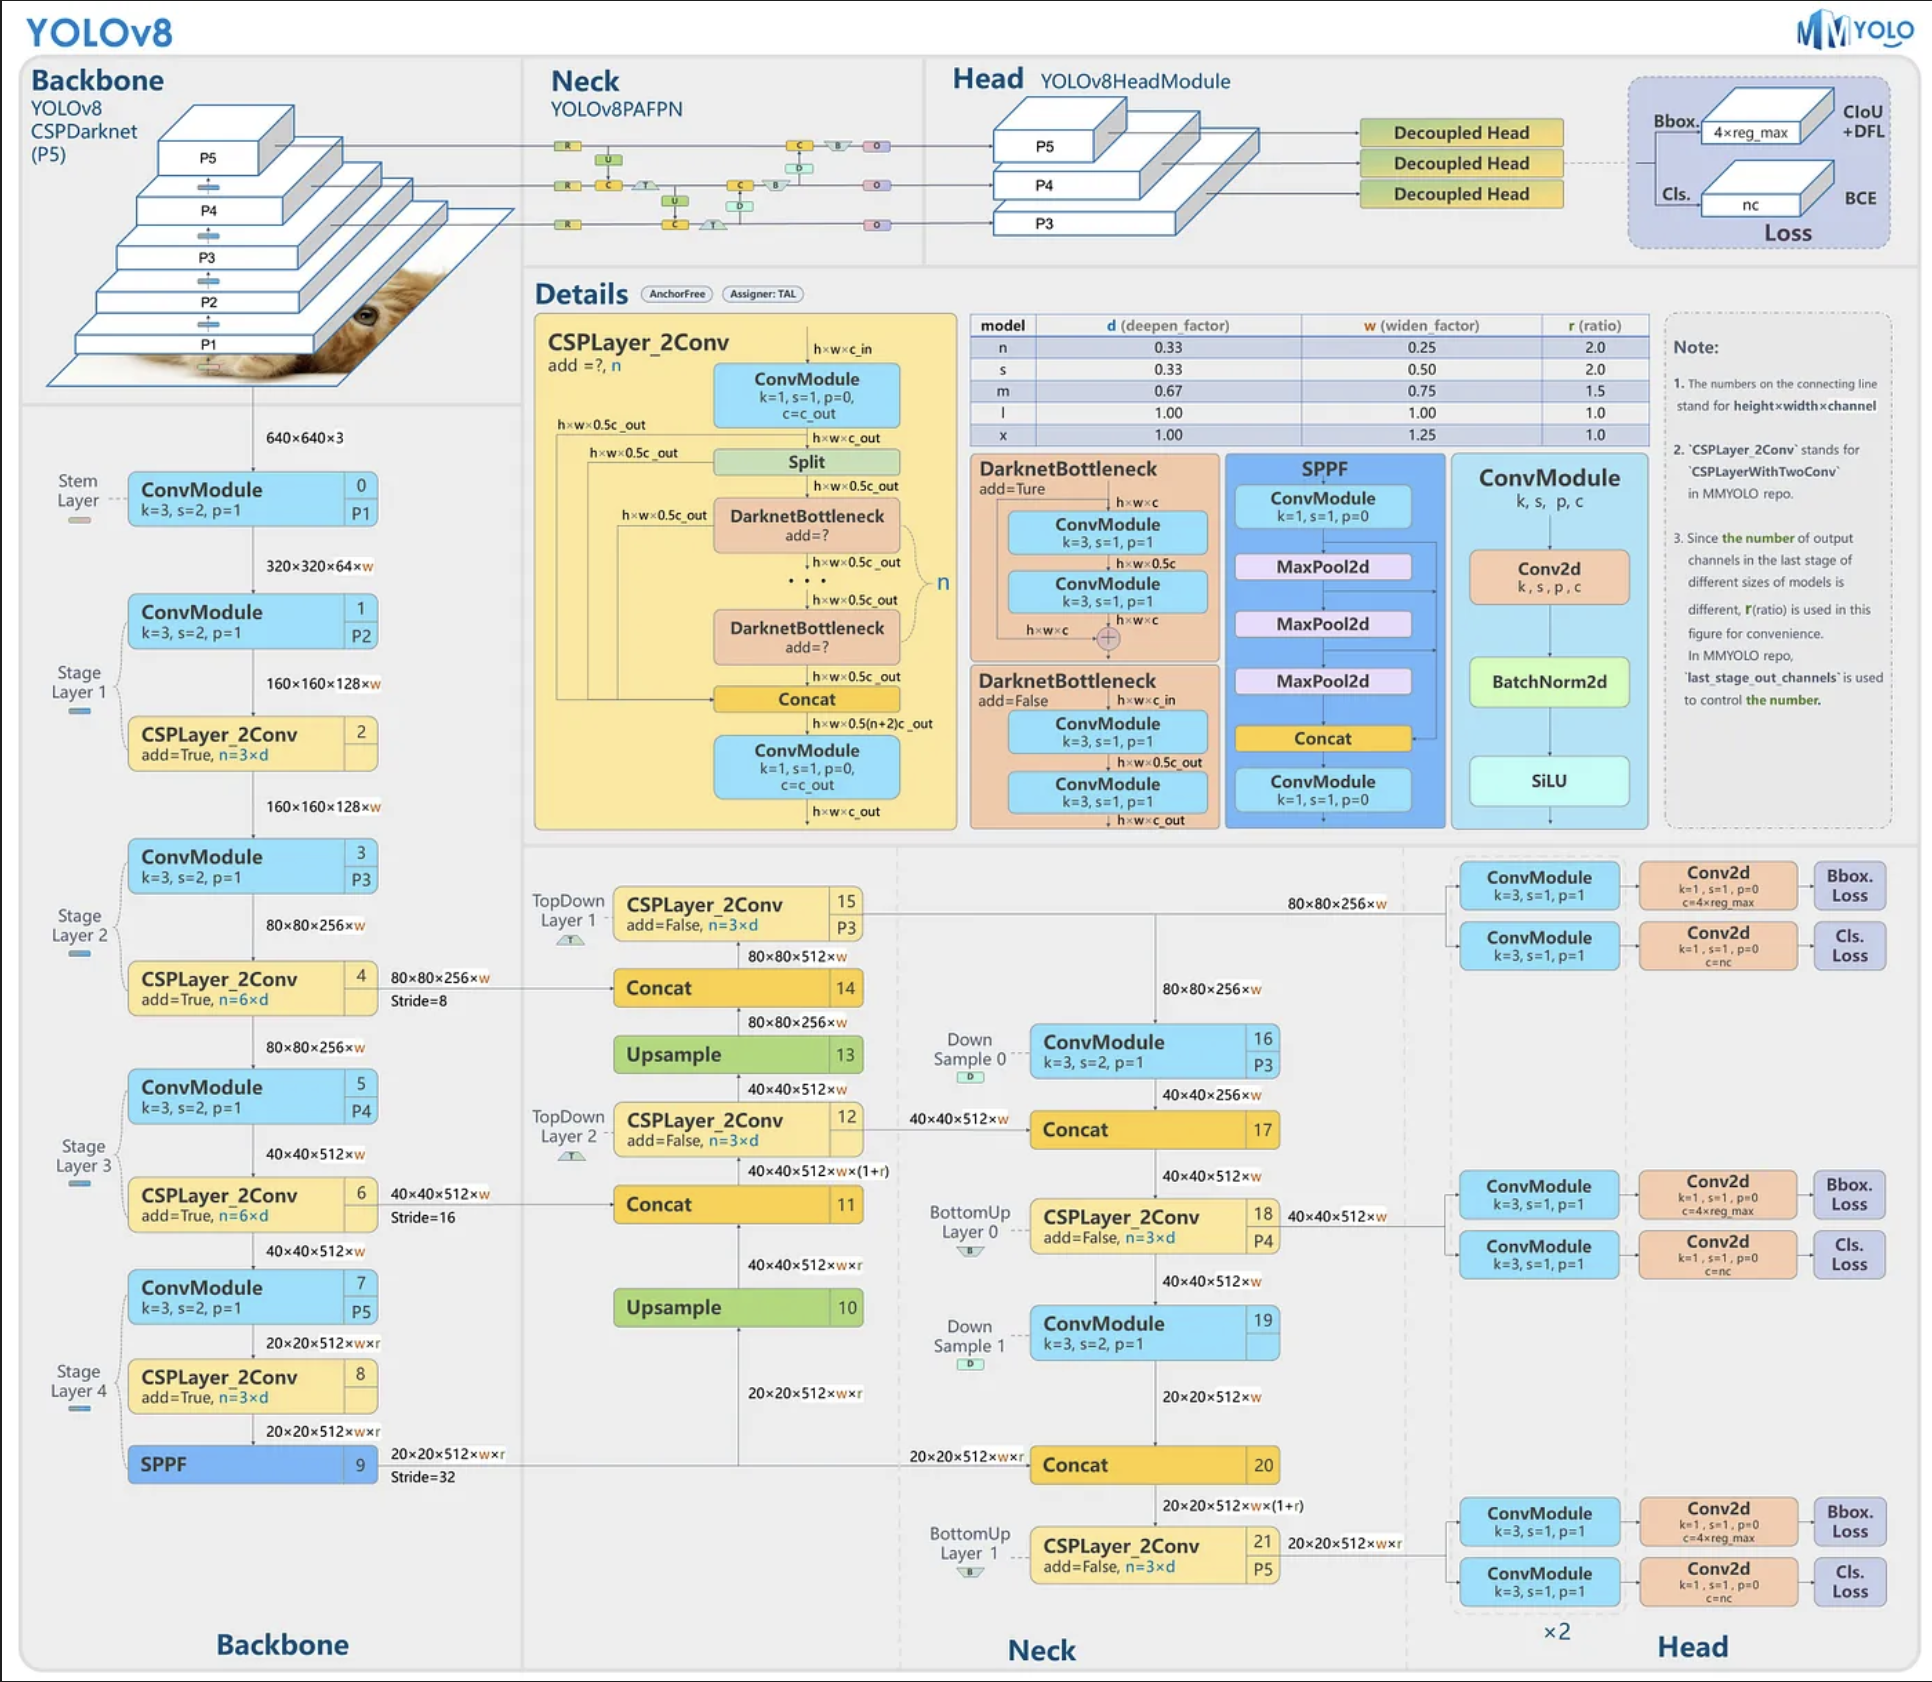
\includegraphics[width=0.9\textwidth]{../img/yolov8-arq3.png}
    \caption{Ilustración detallada de la arquitectura del modelo YOLOv con el Neck y Head separados. \cite{yolov8-arq-neck}}
    \label{fig:YOLOv8_architecture_neck_head}
\end{figure}

% Anadir figura de arquitectura de yolov8 con Neck y Head
%\begin{figure}[H]
%    \centering
%    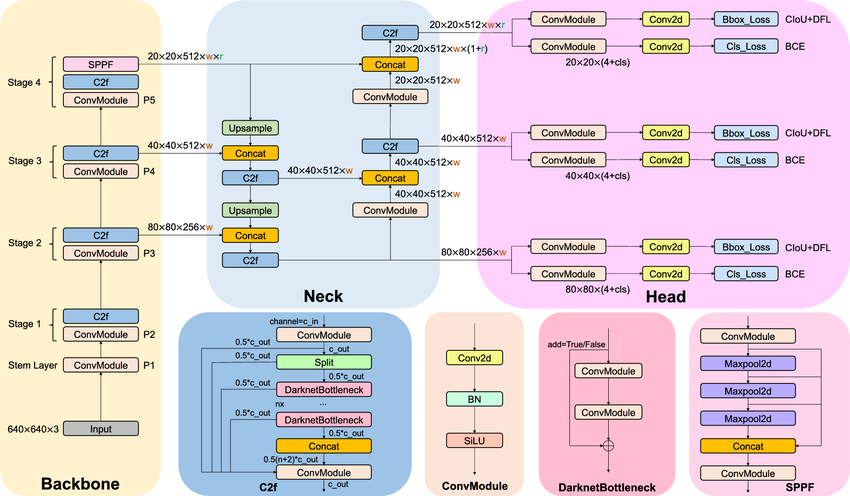
\includegraphics[width=1\textwidth]{../img/yolov8-arq2.png}
%    \caption{Ilustración detallada de la arquitectura del modelo YOLOv8. El Backbone, Neck y Head %son las tres partes de YOLOv8, y C2f, ConvModule, DarknetBottleneck y SPPF son módulos. \cite%{Arquitectura_YOLOv8}}
%    \label{fig:YOLOv8_architecture_neck_head}
%\end{figure}